% =====================================================================
%  c01.tex ------ §1 引言与纲要（原文 pp.3--11，末尾一句续至 p.12 顶部；Lead 撰写）
%  编号公式：1.1--1.10（其中 1.2、1.6 为图形公式，按原 PDF 渲染截取）
% =====================================================================
\section{引言与纲要}
% [原文 p.3]

量子场论（QFT）可以由许多不同的构造产生：拉氏量描述、维数约化、几何工程等等。
由此得到的构件还可以进一步形变（例如部分 Higgs 化）、相互耦合（例如把对称性规范化），或者通过解耦某个子部门而约化。
生活在不同维数中的理论也可以富有成效地耦合在一起。

我们在 4d $\cN=2$ 超对称理论的世界里探索这些构造以及一些计算技术，特别是 class S 理论 [1]，
它们是某个 6d 理论的维数约化（“S” 代表 “Six”）。
class S 包含最常被研究的 4d $\cN=2$ 拉氏量规范理论（超 Yang--Mills（SYM）、超 QCD（SQCD）、箭图规范理论、
$\cN=4$ SYM 及其质量形变）与 Argyres--Douglas（AD）理论 [2] 这样的非拉氏量理论，
也包含大量此前未知的理论------它们大大拓宽了已知 4d $\cN=2$ 理论的范围。

要构造一个 class S 理论，我们从 6d $\cN=(2,0)$ 超共形场论（SCFT）出发，记作 $\cX(\fg)$，
它由单连通（simply-laced）\footnote{一个单李代数 $\fg$ 称为单连通的（simply-laced），如果它所有根的长度相同。
这类代数有 ADE 分类：具体说来，$\fg$ 是 $\fsu(N)$、$\fso(2N)$、$\mathfrak{e}_6$、$\mathfrak{e}_7$ 或 $\mathfrak{e}_8$ 之一。}
李代数 $\fg$ 刻画，例如 $\fsu(N)$。
然后把 $\cX(\fg)$ 在黎曼面 $C$ 上约化（$C$ 称为紫外（UV）曲线\footnote{二维黎曼面 $C$ 是一条复曲线：它的复维数为 1。}），
并借助一套称作\textbf{部分拓扑扭曲}的程序保持 4d $\cN=2$ 超对称性。
黎曼面上可以有穿刺点（即被挖掉的点，于是 $C=\overline{C}\setminus\{z_1,\dots,z_n\}$，其中 $\overline{C}$ 紧致），
在穿刺点处必须给定边界条件。每选定一个带穿刺点的黎曼面，以及描述 $z_i$ 处边界条件的数据 $D_i$，
就得到一个 4d $\cN=2$ class S 理论 $\mathrm{T}(\fg,C,D)$。

由于这些理论有 6d 起源，class S 理论的非微扰动力学被编码在 $C$ 的几何中。
例如，一个理论的 Seiberg--Witten（SW）曲线 [3, 4]------它决定给定 Coulomb 分支真空中的低能有效作用量------就是 $C$ 的一个分歧覆盖。
引人注目的是，这一想法可以推广到 class S 理论的许多可观测量。
AGT 对应 [5] 所关心的正是四球（以及椭球）配分函数：
% [Tutor Note: p.3 式 (1.1) 的右端是 Toda CFT 的顶点算子关联函数；注意上标 Toda(g) 在这一阶段是
% 记号上的“占位”：g = su(2) 时它退化为 Liouville CFT，g 为一般单连通李代数时才真正是 Toda CFT。
% 原文在 1.2 与第 6、7 节逐步把这个记号落实。核对要点：右端只依赖穿刺数据 D_i 与局部坐标 z_i。]
\begin{equation}
  Z_{S^4_b}\bigl(\mathrm{T}(\fg,C,D)\bigr)
  = \Bigl\langle \widehat{V}_{D_1}(z_1)\cdots \widehat{V}_{D_n}(z_n) \Bigr\rangle_{C}^{\mathrm{Toda}(\fg)}
  \tag{1.1}
\end{equation}
其中右端是 Liouville CFT（当 $\fg=\fsu(2)$ 时）或其推广------Toda CFT------中顶点算子的关联函数。
顶点算子插在每一个穿刺点 $z_i$ 处，并依赖于刻画穿刺点的数据 $D_i$。

引言余下部分将快速概述本综述：读者尽可直接跳到正文。
第 2、3、4 节（在 1.1 小节中概述）描述理论 $\mathrm{T}(\fg,C,D)$ 与穿刺数据 $D_i$。
第 5、6 节（在 1.2 小节中概述）解释如何定义并计算 (1.1) 的两端，即 $Z_{S^4_b}$ 与 Liouville CFT 关联函数。
最后，第 7、8、9、10 节描述该对应关系的众多推广，并给出文献指引。
在 1.3 小节中我们列出与 AGT 相关的既有综述。\footnote{欢迎提供（2020 年 1 月 31 日之前发表的）文献，以及关于较新进展的评论。}

% ---------------------------------------------------------------------
\subsection{Class S 理论}
% [原文 p.4]

在正文中我们研究 6d $(2,0)$ 理论 $\cX(\fg)$（第 2 节）、它到 class S 理论的扭曲维数约化（第 3 节），
以及其中某些 4d $\cN=2$ 理论的拉氏量描述（第 4 节）。这里我们只给出这些讨论的一些结论。
为简单起见我们常约化到 $\fg=\fsu(N)$，但到 $\fg=\fso(2N)$ 的推广也已被很好地理解 [6, 7]。

\para{$\mathrm{T}(\fg,C,D)$ 的构件。}
亏格为 $g$、带 $n$ 个穿刺点的黎曼面 $C$ 可以切成 $2g-2+n$ 个三穿刺球面，
后者也称 trinion 或“裤子”\footnote{对带 0、1、2 个穿刺点的球面以及不带穿刺点的环面，这个数目是零或负数：
这些黎曼面不能切成三穿刺球面，class S 构造也不会给出 4d 理论，见 [8]。}，
它们由连接成对穿刺点的管子粘合起来。这样的描述常称为 $C$ 的\textbf{裤子分解}。
相应地，一般的 class S 理论 $\mathrm{T}(\fg,C,D)$ 可以分解为对应每个三穿刺球面的 class S 理论，称为 \textbf{tinkertoy}
（tinkertoy 的复杂度从自由超多重态一直到此前未知的非拉氏量孤立 SCFT）。
每个穿刺点联系着一个味对称性；用管子连接两个穿刺点，就相当于把两个相应的味对称性等同起来并用同一个
4d $\cN=2$ 矢量多重态将它们规范化。例如一个四穿刺球面可以拆成两个三穿刺球面（对合适的群 $G_1,\dots,G_5$）：
% [Tutor Note: 式 (1.2) 是示意图，按原文矢量图 400 dpi 渲染截取，编号随图保留在原图内。
% 图中 “⊗_{gauge G_5}” 表示把两边各自的 G_5 味对称性等同并规范化（即“收缩”一条管子）。
% 两端分别对应两个三穿刺球面的 tinkertoy：左端是四穿刺球面，右端是两个三穿刺球面。]
\begin{equation*}
  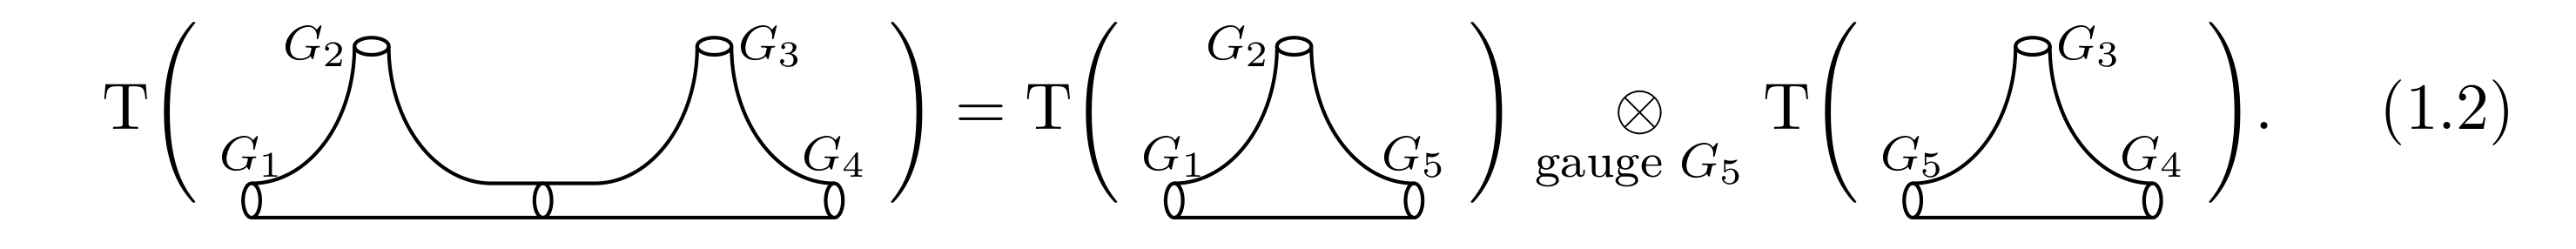
\includegraphics[width=\textwidth]{eq12.png}
\end{equation*}

在 tinkertoy 就是一堆超多重态的简单情形下，这给出由超多重态与矢量多重态构成、具有显式拉氏量的规范理论。

由于部分拓扑扭曲，4d 理论不依赖于 $C$ 的度规 [8, 9]，而只依赖于 $C$ 的复结构；后者可由每根管子的“长度”与“角度”描述。
这两个参数控制着\textbf{复化规范耦合}（$q=\ee^{2\pi\ii\tau}$，其中 $\tau=\frac{\theta}{2\pi}+\frac{4\pi\ii}{g^2}$），
它把对应于该管子的 4d 矢量多重态的 Yang--Mills 耦合 $g$ 与 theta 角 $\theta$ 合并在一起。
弱耦合 $g\to 0$ 对应于很长的管子。
% [Tutor Note: 这里 τ 的约定（τ = θ/2π + 4πi/g²）是全文其余部分的基础，务必与原文一致：
% 若某处出现 q = e^{2πiτ} 与 q̄ 的配对（如 (1.7) 的 Z_cl 因子化），用的正是该约定。
% 易错点：不同文献把 4πi/g² 写成 iθ/(2π) 或 i/(2π g²) 等，跨文献比较公式时必须先统一。]

当然，$C$ 可以有许多种三穿刺球面分解；相应地，$\mathrm{T}(\fg,C,D)$ 有许多涉及完全不同的场与规范群的等价对偶描述。
这些描述的弱规范耦合区域，对应于 $C$ 上复结构可由某个裤子分解（其中三穿刺球面由很长的管子相连）很好地描述的区域。
这些区域是 $C$ 的复结构空间的不同尖点（cusp），它们通过改变规范耦合而连续相连。
这样一来，一种描述中的强耦合规范理论可能具有另一种弱耦合描述。
这一现象 [1] 推广了 $SU(2)$ $N_f=4$ 理论与 $\cN=4$ SYM 的 S 对偶。
于是 6d 构造通过 $C$ 使这些 S 对偶变得显然。

% [原文 p.5]
在 6d 构造中，位于 $z_i\in\overline{C}$ 的穿刺点是绕 class S 理论所定义之 4d 时空的余维 2 缺陷。
为保持 4d 理论的超对称性，这些缺陷应是半 BPS 的，即保持原超对称性的一半。
必须对这类缺陷进行分类（通常沿 Coulomb 分支移动来进行），然后再对三穿刺球面对应的 tinkertoy 分类。
顺带一提，6d 理论还容许支撑在 2d 子空间上的、有趣的半 BPS 余维 4 算子，它们丰富了这一对应关系。

\para{Coulomb 分支与 Seiberg--Witten 曲线。}
把握理论 $\mathrm{T}(\fg,C,D)$ 的一条途径，是描述其超对称真空（尤其是其 Coulomb 分支），并给出理论在每个真空附近的低能行为。
这个分支由 \textbf{Coulomb 分支算子}张成，即被所有 4d 反手征超荷湮灭的局域算子。

半经典地，6d $(2,0)$ 理论 $\cX(\fg)$ 的真空在模去规范变换后，由一些（对易、可对角化的）伴随值标量 $\Phi_I$ 参数化，
其中 $I=6,\dots,10$ 是 $\fso(5)$ R 对称性\footnote{在 6d 理论的 M 理论构造中，$\fso(5)$ 转动坐标 $x^6,\dots,x^{10}$。}的指标。
或者，它们可以由规范不变多项式（Casimir）如 $\Tr(\Phi_I\Phi_J)$ 的（相容的）取值来参数化。
4d 理论的 Coulomb 分支真空，则是那些允许沿曲线 $C$ 变化的 $\Phi_I$（更确切地说是不变多项式）的构型。
更准确地说，追查 4d $\cN=2$ 反手征超荷如何嵌入 6d $\cN=(2,0)$，我们得到两条限制：
Casimir 全纯地依赖于坐标 $z\in C$；并且在所有 $\Phi_I$ 中只有 $\Phi_z:=\Phi_6+\ii\Phi_7$ 非零。
由于部分拓扑扭曲把 R 对称性的一个子代数 $\fso(2)$（$\Phi_z$ 在其下带荷）混入 $C$ 上的转动群，
$\Phi_z\dd z$ 在 $C$ 上是张量性的（具体说是一个 1-形式）。
粗略地说，4d Coulomb 分支由 $C$ 上伴随值全纯 1-形式 $\Phi_z\dd z$（模去规范变换）参数化，
更不变量地说，由 Casimir 多项式的真空期望值（VEV）$\langle P_k(\Phi_z)\rangle \dd z^k$ 参数化。

在 $\fg=\fsu(N)$ 的情形，我们把它们重新打包为 $\phi_k(z)=u_k(z)\dd z^k$，$k=2,\dots,N$，
其定义是：在局部坐标 $z\in C$ 中展开
% [Tutor Note: (1.3) 是 su(N) 情形 Coulomb 分支的核心关系。核对要点：右端首项 x^N 的系数为 1
% （即 det(x−Φ_z) 是首一的），求和从 k = 2 起------k = 1 项因 su(N) 无迹而缺失。
% 若在某处看到 k = 1 的项，那它属于 u(N) 情形，对应额外的一个 U(1) 因子。]
\begin{equation}
  \langle \det(x-\Phi_z) \rangle
  = x^N + \sum_{k=2}^{N} u_k(z)\, x^{N-k}.
  \tag{1.3}
\end{equation}
于是考虑这个行列式的零点是有用的：
\begin{equation}
  \Sigma=\Bigl\{(z,x)\ \Big|\ x^N+\sum_{k=2}^{N}u_k(z)x^{N-k}=0\Bigr\}\subset T^*C,
  \tag{1.4}
\end{equation}
其中 $z$ 是 $C$ 上的坐标，$x$ 参数化余切丛 $T^*C$（即 $C$ 上 1-形式丛\footnote{这只是说 $x\dd z$ 在 $C$ 上作坐标变换时按张量变换。}）的纤维。
复曲线 $\Sigma$ 依赖于真空的选取（由 $\phi_2,\dots,\phi_N$ 指定），结果正是 $\mathrm{T}(\fg,C,D)$ 的 SW 曲线，
它表现为 $C$ 的 $N$ 重（分歧）覆盖。它天然配有 1-形式 $\lambda=x\dd z$，即 SW

% [原文 p.6]
微分\footnote{式 (1.4) 常改写为 $\lambda^N+\sum_{k=2}^{N}\phi_k(z)\lambda^{N-k}=0$。}。
由给定 Coulomb 分支真空中 $\mathrm{T}(\fg,C,D)$ 的 SW 曲线与微分 $(\Sigma,\lambda)$，可以导出红外有效作用量（预势）。
BPS 粒子的质量也可以表示为 $\lambda$ 沿闭合围道的积分。

\para{驯服穿刺与 tinkertoy。}
在这一语言中，位于 $z_i\in\overline{C}$ 的穿刺点被描述为规范不变量 $\phi_k$ 的奇点。
一个重要例子是\textbf{满驯服穿刺}（full tame puncture）：它在 $z_i$ 处（在共轭意义下）要求一阶极点
$\Phi_z\sim m_i(z-z_i)^{-1}\dd z+O(1)$，其中留数 $m_i$（属于 $\fg$ 的复化 $\fg_{\C}$）是适当一般的元素。
这个质量\footnote{对 $\fsu(N)$，$m_i$ 的 $N$ 个本征值给出 $\lambda$ 在 $\Sigma$ 上投影到 $z_i$ 的 $N$ 个点处的留数。
对 $\lambda$ 积分以计算 BPS 粒子质量时会拾取这些留数，故它们正是质量参数。}参数 $m_i$ 可以理解为
耦合到 $z_i$ 处穿刺所对应味对称性 $\fg$ 的\textbf{背景}矢量多重态标量的常数值。
用规范不变的语言，这个一阶极点转化为
\begin{equation}
  \langle P_k(\Phi_z)\rangle = \frac{P_k(m_i)}{(z-z_i)^k}+\cdots,
  \tag{1.5}
\end{equation}
或等价地 $\phi_k\propto \dd z^k/(z-z_i)^k+\cdots$，其首项系数由 $m_i$ 确定（在 $\fsu(N)$ 情形用 (1.3)）。

事实上，当 $C$ 被捏紧并在一根管子变得无限细的极限下分裂为二时，这类奇点一般地会出现。
因此 class S 理论的主要构件是 tinkertoy $T_{\fg}$，即联系着带三个满驯服穿刺点的球面的理论。
常用记号 $T_N:=T_{\fsu(N)}$。通过把 $\mathrm{T}(\fsu(2),C,D)$ 理论的 SW 曲线与 SW 微分同已知理论（如 $SU(2)$ $N_f=4$ SQCD）对照，
可以验证 $T_2$ 不过就是 4 个自由超多重态的集合 [1]。
但一般地，理论 $T_{\fg}$ 是非拉氏量理论，每个穿刺点（至少）带一个味对称性 $\fg$。
例如 $T_{\fsu(3)}$ 是味对称性为 $\mathfrak{e}_6\supset\fsu(3)^3$ 的 Minahan--Nemeschansky SCFT。
% [Tutor Note: 这里的 su(3)^3 不是笔误：T_su(3) 的三个满驯服穿刺各携带一个 su(3)，故味对称性为 su(3)^3；
% 而 SU(3)^3（秩 6）正是 E6 的极大子群，与 e6 的总秩 6 相符。核对方法：数穿刺点（3 个）× 每点 su(3) 的秩（2）= 6 = rank E6。]

还存在更一般的驯服穿刺：在那些点上要求 $\Phi_z$ 的一阶极点，但留数 $m$ 可以非一般。
由此得到的 tinkertoy 相当于部分 Higgs 化：通过给穿刺所携带对称性（的矩映射）打开一个幂零 VEV，
移动到 $T_{\fg}$ 的 Higgs 分支上，从而降低对称性。
% [Tutor Note: “部分 Higgs 化 = 沿 Higgs 分支移动”这一句是理解 [N−1,1] 类穿刺的钥匙：
% 幂零 VEV 的轨道由 N 的分拆分类（Spaltenstein/Springer 对应），每个分拆给出一个幂零轨道，
% 从而给出不同的味对称性破缺模式。分拆 [1^N] 对应满驯服穿刺（su(N) 味对称性完好），[N] 对应“无穿刺”。]
对 $\fsu(N)$，它们由 $m$ 的本征值相等模式刻画，编码为 $N$ 的一个分拆，并导致 $\phi_k$ 的更低阶极点。
满驯服穿刺对应的分拆是 $N=1+1+\cdots+1$，也记作 $[1^N]$；它携带 $\fsu(N)$ 味对称性（被质量 $m$ 显式破缺）。
另一极端，对应分拆 $[N]$（所有本征值相等，故 $m=0$）的穿刺是“无穿刺”的平凡情形，因为它是留数为零的极点。
下一个“最小”的穿刺称为\textbf{单驯服穿刺}（simple tame puncture），对应分拆 $[N-1,1]$，
于是 $m=\diag(m_1,\dots,m_1,-(N-1)m_1)$；它携带 $\mathrm{U}(1)$ 味对称性，$N=2$ 时增强为 $\fsu(2)$，
因为此时单驯服穿刺与满驯服穿刺相同。满驯服穿刺与单驯服穿刺都出现在 $SU(N)$ $N_f=2N$ SQCD 的 class S 描述中，
如图 1 所示。
% [Tutor Note: 核对 m 的无迹性：diag(m1,…,m1,−(N−1)m1) 的迹为 (N−1)m1−(N−1)m1=0，确实属于 su(N)。
% 这一“一阶极点 + 幂零留数 = 分拆”的对应关系在 §7.3（野生穿刺）中会被推广为高阶极点。]
\begin{figure}[htbp]
\centering
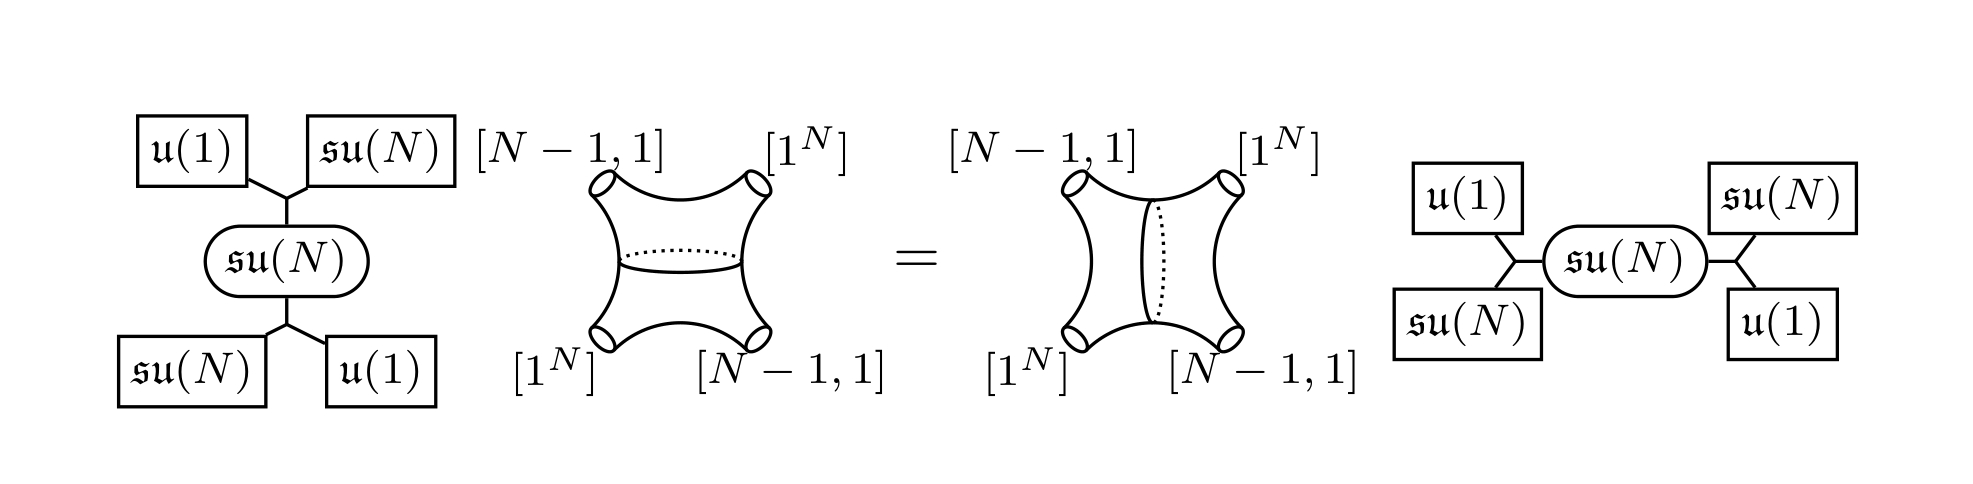
\includegraphics[width=0.75\textwidth]{fig1.png}
\figtitle{1}{对应带两个满驯服穿刺点（标记 $[1^N]$，味对称性 $\fsu(N)$）与两个单驯服穿刺点（标记 $[N-1,1]$，
味对称性 $\mathrm{U}(1)$）的球面的 $\fsu(N)$ class S 理论。图中画出由“一个单驯服 + 两个满驯服”穿刺的球面构成的两个裤子分解，
其对应的 tinkertoy 是一堆超多重态。这两个分解给出该理论作为 $SU(N)$ $N_f=2N$ SQCD 的两种 S 对偶拉氏量描述。
第三个裤子分解（图中未画）涉及非拉氏量 tinkertoy（当 $N>2$ 时）。}
\end{figure}

% [原文 p.7]
当所有穿刺点都是满驯服穿刺时，每根管子所携带的规范代数为 $\fg$；更一般的驯服穿刺则可能导致更小的规范代数。
例如，$\fsu(N)$ class S 包含规范群为 $\prod_i SU(N_i)$（其中 $N_i\le N$）的线性箭图规范理论，
每个双基本表示 $N_i\otimes N_{i+1}$ 中有一个超多重态，每个 $SU(N_i)$ 的基本表示 $N_i$ 中有
$M_i\le 2N_i-N_{i-1}-N_{i+1}$ 个超多重态\footnote{当此界饱和时，该群的规范耦合不跑动。
当它被满足但不饱和（即 $M_i<2N_i-N_{i-1}-N_{i+1}$）时，我们得到渐近自由规范理论，它可以用野生穿刺在 class S 中实现。
反之，当此界被违反时，该理论只是有效理论，没有 class S 构造。}。这概括在箭图
% [Tutor Note: (1.6) 是示意图，按原图 500 dpi 渲染截取，编号随图保留。
% 箭图约定：圆角节点 = SU(N_i) 规范群，方框节点 = M_i 个基本超多重态，
% 相邻节点间的连线 = 一个双基本超多重态。]
\begin{equation}
  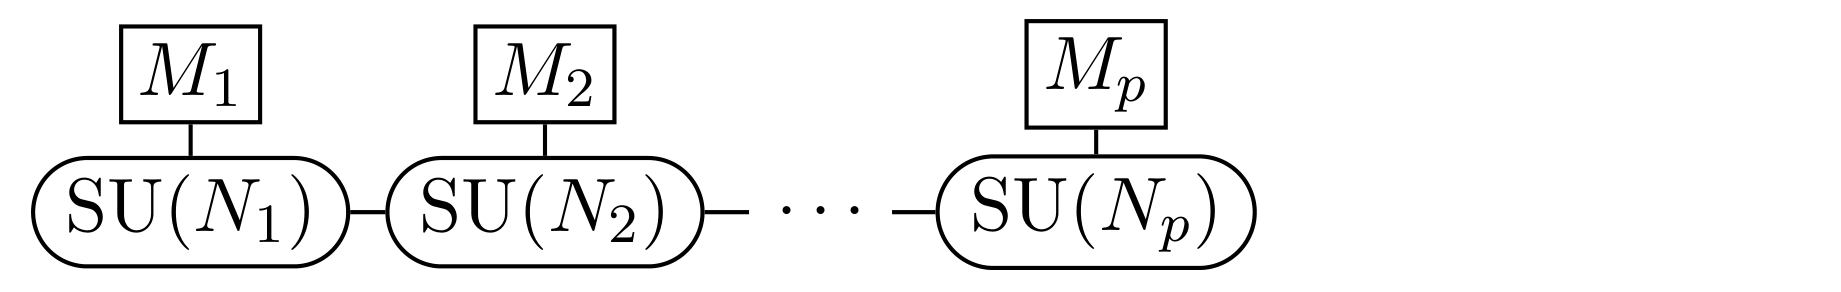
\includegraphics[width=0.59\textwidth]{eq16.png}
  \tag{1.6}
\end{equation}

% ---------------------------------------------------------------------
\subsection{基本 AGT 对应}
% [原文 p.7]

这里我们概述为此后完整 AGT 对应作铺垫的两节内容。
首先，第 5 节描述如何用超对称局域化计算箭图规范理论的（压扁）球面配分函数 $Z_{S^4_b}$，尤其是瞬子计数问题。
然后，第 6 节解释 Liouville CFT 的基本方面，并给出 $\fg=\fsu(2)$ 广义箭图情形下 AGT 对应的精确陈述。

\para{超对称局域化。}
在第 5 节中我们解释如何把 class S 理论超对称地放到（压扁的）四球
$S^4_b:=\{y_5^2+b^2(y_1^2+y_2^2)+b^{-2}(y_3^2+y_4^2)=r^2\}\subset\R^5$ 上，
这顺便还要求质量取纯虚数。我们还解释如何用超对称局域化 [10, 11] 在这个椭球上计算配分函数。
这一路径积分技术适用于 $\mathrm{T}(\fg,C,D)$ 的每一种 4d $\cN=2$ 拉氏量描述------如果存在这样的描述的话。\footnote{我们在切割黎曼面时发现的 $Z_{S^4_b}$ 的因子化性质，对非拉氏量 class S 理论也成立。
它们是对矢量多重态（而非 tinkertoy）应用超对称局域化得到的。}
超对称局域化可以

% [原文 p.8]
把无穷维路径积分约化为在超多重态与矢量多重态的某个超对称构型上的有限维积分。
人们发现，这些构型由矢量多重态标量的（纯虚）常数值 $a$ 标记，$a$ 可经规范固定取在规范代数的 Cartan 子代数中。
这些构型还被 $S^4_b$ 一个极点（$y_5=r$）处的点状瞬子
与另一极点（$y_5=-r$）处的反瞬子所“修饰”。于是配分函数为
\begin{equation}
  Z_{S^4_b}(q,\bar q)=\int \dd a\, Z_{\mathrm{cl}}(a,q,\bar q)\, Z_{\mathrm{one\text{-}loop}}(a)\,
  Z_{\mathrm{inst}}(a,q)\, Z_{\mathrm{inst}}(a,\bar q),
  \tag{1.7}
\end{equation}
其中我们省略了对 $\fg$ 与穿刺数据 $D$ 的依赖，但显式写出对曲线 $C$ 的复结构参数 $q$ 的依赖。
这里 $Z_{\mathrm{cl}}$ 来自超对称构型的经典作用量；它非全纯地依赖于复规范耦合 $q$，但可因子化为
$Z_{\mathrm{cl}}(a,q,\bar q)=Z_{\mathrm{cl}}'(a,q)Z_{\mathrm{cl}}'(a,\bar q)$。
对这些构型作二次涨落给出 $Z_{\mathrm{one\text{-}loop}}(a)$，它是特殊函数的一个直截了当的乘积，完全与 $C$ 的形状（复结构）无关。
最后，每个极点处的（反）瞬子带来一个因子 $Z_{\mathrm{inst}}$，它（反）全纯地依赖于规范耦合 $q$。
% [Tutor Note: (1.7) 的因子化是 AGT 对应“半边”结构的体现：Z_cl 与 Z_inst 只依赖 q（全纯），
% 其复共轭只依赖 q̄（反全纯），而 Z_one-loop 与 q 无关。第 6 节把它逐因子对到 Liouville 侧：
% Z_one-loop = C(μ,α)、Z_cl' Z_inst = F(μ,α,q)。核对要点：这里 a（矢量多重态标量）与 Liouville 侧的内部动量 α 对应，且 a 为纯虚数。]

因子 $Z_{\mathrm{inst}}(a,q)=\sum_{k\ge 0}q^k Z_{\mathrm{inst},k}(a)=1+O(q^1)$ 是 Nekrasov 瞬子配分函数 [12, 13]，
参数为 $\epsilon_1=b/r$、$\epsilon_2=1/(rb)$，在有利情形下可计算。
主要困难在于计算每一份 $k$-瞬子贡献 $Z_{\mathrm{inst},k}(a)$，它是 $k$-瞬子模空间上的积分。
该空间是有限维的但非常奇异，其奇点对幺正规范群理解得最好。
对于幺正群的线性箭图（由 (1.6) 把所有 $SU(N_i)$ 规范群替换成 $U(N_i)$ 得到），
Nekrasov 配分函数可由等变局域化或 IIA 膜构造确定。
于是我们关心的 $SU$ 理论 (1.6) 的瞬子配分函数，可通过适当解耦 $U(1)$ 因子（即把 $Z_{\mathrm{inst}}(a,q)$
除以 $(1-q)$ 的幂这样的简单因子）来导出 [5]。
人们还设计了各种其他方法，但对一般 class S 理论的 $Z_{\mathrm{inst}}$，迄今仍没有完整的第一性原理推导，
即使限制到带驯服穿刺的 $\fg=\fsu(2)$ 也是如此。\footnote{感谢 Jaewon Song 就这一点所作的澄清。}

若 S 对偶成立，同一理论由 $C$ 的不同裤子分解得到的对偶拉氏量描述应有相同的配分函数。
要证明显式积分表达式 (1.7) 的相等是极其困难的，即使对 $SU(2)$ $N_f=4$ 理论也是如此。
事实上，我所知最简单的办法是在该情形下推导 AGT 对应（例如 [14]），再依赖 [15--17] 所示 2d CFT 侧的模性质。

\para{Liouville CFT 关联函数与基本 AGT 对应。}
在第 6 节中我们转向 $\fg=\fsu(2)$ 情形对应的另一边，即 Liouville CFT 的关联函数。
Liouville CFT 依赖于“背景荷” $Q=b+1/b\ge 2$（中心荷为 $c=1+6Q^2\ge 25$），
它在 4d 侧对应椭球 $S^4_b$ 的一个形变参数。
% [Tutor Note: 这里的 Q = b + 1/b 与 c = 1 + 6Q² 是 Liouville CFT 的标准约定（b 为耦合常数，c ≥ 25）。
% 易错：不少文献把 Q 记作 b + 1/b，也有些用 c = 13 + 6Q² 的写法------但那是 N=2 超 Liouville 的中心荷，
% 与普通 Liouville 的 c = 1 + 6Q² 不是同一个理论，不能相互替换。跨文献对照共形权
% h(α) = α(Q−α) 与中心荷时必须先固定约定。]

% [原文 p.9]
如同任何 2d CFT，局域算子组织成共形族，后者由 Virasoro 代数作用在主算子上生成。
在 Liouville CFT 中，这些主算子是顶点算子 $\widehat{V}_\alpha$，由一个连续参数 $\alpha=Q/2+\ii P$ 标记，
其中 $P\in\R/\Z_2$（称为\textbf{动量}）；它们有相等的全纯与反全纯维数
$h(\alpha)=\alpha(Q-\alpha)=Q^2/4+P^2$。
在 $\fsu(2)$ 情形，每个驯服穿刺的数据 $D_j$ 约化为指定一个质量 $m_j\in\ii\R/\Z_2$（纯虚），
自然地与一个 Liouville 动量等同（相差球面半径 $r$）：AGT 对应于是断言
\begin{equation}
  Z_{S^4_b}\bigl(\mathrm{T}(\fsu(2),C,m)\bigr)
  =\Bigl\langle \widehat{V}_{Q/2+rm_1}(z_1)\cdots \widehat{V}_{Q/2+rm_n}(z_n)\Bigr\rangle_{\overline{C}}^{\mathrm{Liouville}}.
  \tag{1.8}
\end{equation}
如同任何 2d CFT，黎曼面 $\overline{C}$ 上 Virasoro 主算子的 $n$-点函数，对带穿刺黎曼面 $C$ 的每一种裤子分解都有一个有用的表达式。
其想法是沿分解的每条割线插入一组完备态，然后利用 Virasoro 对称性把所有出现的三点函数用主算子的三点函数改写。
示意地，这给出
% [Tutor Note: (1.9) 中 C(μ,α) 是 Liouville 结构常数的组合（具体是 DOZZ 公式给出的三点函数系数），
% F(μ,α,q) 是共形块。对照 (1.7) 时应把 Z_cl' Z_inst 与 F 对应、Z_one-loop 与 C 对应。]
\begin{equation}
  \Bigl\langle \widehat{V}_{\mu_1}(z_1,\bar z_1)\cdots \widehat{V}_{\mu_n}(z_n,\bar z_n)\Bigr\rangle_{C}^{\mathrm{Liouville}}
  =\int \dd \alpha\, C(\mu,\alpha)\,\cF(\mu,\alpha,q)\,\overline{\cF(\mu,\alpha,\bar q)}.
  \tag{1.9}
\end{equation}
这里我们对所有内部动量 $\alpha$ 积分，$\alpha$ 标记每一组插入完备态中的共形族。
因子 $C(\mu,\alpha)$ 是 Liouville CFT 结构常数的组合。
另外两个因子是\textbf{共形块}，它们纯粹关乎 Virasoro 代数的表示论，
并（反）全纯地依赖于 $C$ 的复结构参数 $q$，其中包含 $z_i$ 的（交比）。

AGT 对应的两端对 $C$ 的每种裤子分解都容许形式相同的表达式 (1.7) 与 (1.9)：
每根管子对应一个积分变量 $a$ 或 $\alpha$，并且对 $q$ 的依赖因子化为全纯与反全纯两部分。
事实上，这两个表达式逐因子相配：$Z_{\mathrm{one\text{-}loop}}(m,a)=C(\mu,\alpha)$，且
$Z_{\mathrm{cl}}'(a,q)Z_{\mathrm{inst}}(m,a,q)=\cF(\mu,\alpha,q)$。
这一字典中的另一条款是：在经典极限 $r\to\infty$ 下，4d 侧的 $\phi_2$ 对应于 Liouville 侧的全纯能动张量 $T(z)$：
与 $T(z)$ 的算子乘积展开（OPE）中的首项与 $r^2\phi_2(z)$ 相配，
\begin{equation}
  T(z)\widehat{V}_\mu(0)=\frac{h(\mu)\widehat{V}_\mu(0)}{z^2}+\cdots
  \ \overset{r\to\infty}{\simeq}\ -\frac{r^2m^2}{z^2}\widehat{V}_\mu(0)+\cdots
  \simeq -r^2\phi_2(z)\widehat{V}_\mu(0)+\cdots.
  \tag{1.10}
\end{equation}
我们在第 6 节末尾概述 Liouville CFT 如何在把 6d 理论约化到 $S^4$ 上时出现 [18]。

\para{AGT 对应的推广。}
第 7 节从两方面推广 AGT 对应。
第一，渐近自由理论与 AD 理论通过把驯服穿刺换成野生穿刺来描述，这在 CFT 侧把主顶点算子换成了非正规算子。
第二，$\fsu(2)$ 被换成 $\fg=\fsu(N)$：于是超多重态被换成非拉氏量构件 $T_N$，Liouville CFT 被换成 Toda CFT。

% [原文 p.10]
第 8 节研究如何把各种规范理论算子（局域算子、Wilson--'t Hooft 圈……）纳入 AGT 对应。
CFT 侧出现的是 Verlinde 圈、退化顶点算子、融合核与编织核，以及带边界的黎曼面。
这一字典与相应文献概括在表 1 中。
% [Tutor Note: 表 1 的“余维 4 / 余维 2”分栏指 6d 中产生该算子的缺陷（或轨形）的余维数；
% 第二列是 4d 侧的维数。注意 2d 一行出现两次：涡旋弦算子（余维 4 组）与 Gukov--Witten 面缺陷（余维 2 组）
% 都是 4d 中 2 维的算子，但来源的 6d 缺陷余维不同------这是本表最容易被误读的地方。]
\begin{table}[htbp]
\centering
\small
\renewcommand{\arraystretch}{1.3}
\setlength{\tabcolsep}{4pt}
\begin{tabular}{@{}>{\centering\arraybackslash}m{0.5cm} >{\centering\arraybackslash}m{0.7cm} p{5.5cm} p{4.7cm} p{3.4cm}@{}}
\toprule
 & & class S 理论中的算子 & Liouville/Toda CFT & 文献 \\
\midrule
\multirow{4}{*}{\rotatebox{90}{余维 4}} & 0d & Coulomb 分支算子 & 积分流 & [19] \\
\cmidrule(l){2-5}
 & & 轨形 $\C^2/\Z_M$ & 把 CFT 变为陪集 & [20--37] \\
\cmidrule(l){2-5}
 & 1d & 双荷圈：威尔逊圈 / 't Hooft 圈 & 退化 Verlinde 圈：\newline 绕管子 / 横向 & $\fsu(2)$ [38--44]，\newline $\fg$ [45--54] \\
\cmidrule(l){2-5}
 & 2d & 涡旋弦算子 & 退化顶点算子 & [39, 55--71] \\
\midrule
\multirow{5}{*}{\rotatebox{90}{余维 2}} & 2d & Gukov--Witten 面缺陷，或轨形 $\C\times(\C/\Z_M)$ & 经 Drinfeld--Sokolov 约化改变 CFT & [72--85] \\
\cmidrule(l){2-5}
 & & 破缺对称性的畴壁 & Verlinde 圈 & [43] \\
\cmidrule(l){2-5}
 & 3d & S 对偶畴壁 & 模核（modular kernel） & [86--90] \\
\cmidrule(l){2-5}
 & & 边界 & 边界 CFT & [91, 92] \\
\cmidrule(l){2-5}
 & 4d & 与 tinkertoy 耦合 & 顶点算子 & [5, 93--109] \\
\bottomrule
\end{tabular}
\tabtitle{1}{延伸算子的 AGT 对应。按产生它们的 6d 算子（或轨形）的余维数排序，并在每一组内按 4d 侧的维数排序。
原表中多数条目带有指向正文的超链接。}
\end{table}

我们在第 9 节讨论 AGT 对应的一些分支。
把 6d 理论放到其他乘积空间 $M\times C$（带某种扭曲）上，会给出 $M$ 上的理论与 $C$ 上的理论之间有趣的关系：
指标/qYang--Mills（YM）对应 [110]、3d/3d 对应 [111]、2d/4d 对应 [112]。
另一方向上，某些 class S 理论（尤其是线性箭图规范理论）可以实现为 5d $\cN=1$ 理论的约化。
瞬子配分函数在 5d 中有直接对应物，即 4d 结果的某种 $q$-形变。
这导出一个 $q$-形变的 AGT 对应 [113]，它把这些 5d 瞬子配分函数等同于 $q$-形变 Virasoro 或 $W_N$ 代数的
手征关联函数（“共形块”）。$S^5$ 配分函数涉及三个瞬子配分函数，
它到完整 $q$-Toda 理论非手征关联函数的恰当翻译仍在研究中 [114]。
最后在第 10 节，我们简要列出本综述省略的许多主题，如矩阵模型、拓扑弦、量子可积系统等。

% ---------------------------------------------------------------------
\subsection{既有综述}
% [原文 p.10--11]

与 AGT 对应相关的好综述已经很多，其中一些是博士论文。
我特别推荐 Tachikawa 那套非常清晰的综述 [115--118]。

\begin{itemize}[leftmargin=1.6em,itemsep=2pt]
\item \textbf{6d $(2,0)$ SCFT。}这些理论、以及更一般的 6d $(1,0)$ SCFT，在 [119] 中从 F 理论视角作了综述。
      关于在 AGT 对应中处于核心地位的余维 2 缺陷，见 [120]。
\item \textbf{4d $\cN=2$ 与 Seiberg--Witten。}关于 4d $\cN=2$ 理论的 SW 解，虽然 1990 年代后期有不错的入门 [121, 122]，
      但我更推荐更现代的解释，例如 Martone 在本校的讲义 [123]，以及那篇著名的“面向行人”的综述 [115]------
      它覆盖面很广，包括 AD 理论如何从 SQCD 的极限中出现。书 [124] 讨论了 4d $\cN=2$ 理论与其他主题之间的许多现代联系。
      综述 [117] 聚焦于极重要的非拉氏量 4d $\cN=2$ 理论 $T_N$。
\item \textbf{局域化与瞬子计数。}超对称局域化在书 [125] 中有综述，特别是压扁四球配分函数见 [126]。
      其表达式涉及 Nekrasov 瞬子配分函数，好的起点是 [116]，随后是 [127]------后者讨论了所有规范群、
      关于 $U(1)$ 因子的微妙之处以及重整化方案的选择。
\item \textbf{Toda CFT 与 $W$ 代数。}\footnote{感谢 Ioana Coman 提供指引。}
      Liouville CFT 在许多文献中有综述，如 [128, 129]；关于一些微妙之处，值得读 [130]。
      目前没有关于 Toda CFT 或 $W$ 代数的近期综述。关于 $W$ 代数，可看较旧的 [131, 132]（以及可能的 [133]），
      或 [134, 135] 中 $W_{1+\infty}$ 的截断。关于 Toda CFT，或许可看早期文章 [136] 或我的学位论文 [137]\footnote{非常欢迎更好的文献：那里只考虑了 $A_{N-1}$ 情形，
      而且只涉及满、单与退化穿刺，未涉及以 $N$ 的分拆标记的一般驯服穿刺。}。
\item \textbf{面向物理学家的 AGT。}简短综述见 [118]（或 [138]，日文），更长的综述见 [139]------从 SW 基础一直到由 SQCD 退化产生的 AD 理论。
      AGT 的矩阵模型进路见综述 [140, 141]。
\item \textbf{面向数学家的 AGT。}数学家的可能起点包括入门性讨论班笔记 [142]、
      一篇“伪数学的伪综述” [143, 144]、不完整（但仍有 200 页）的讲义 [145]、该对应的范畴化版本 [146]、
      一篇聚焦平坦联络模空间的综述 [147]，以及一篇讨论渐近局部欧氏（ALE）空间上瞬子计数的综述 [148]。
      还有关于 6d $(2,0)$ SCFT 在几何表示论、辛对偶、纽结同调与 Hitchin 系统中数学应用的笔记 [149]。
\item \textbf{AGT 的推广。}包括 [150] 中综述的 3d/3d 对应，以及 [151] 中 5d $\cN=1$ 规范理论与 $q$-Toda 关联函数之间的 AGT 关系。
\end{itemize}

鉴于已有如此多的综述，再写一套笔记也许是徒劳的；但希望这里采取的相当不同的进路------从 6d 理论出发------
对某些读者来说是合适的。
% [原文 p.12 顶部（本段由 Lead 收尾；其后 “Part I / 第 2 节” 起属 tr-01）]
我为自己在本综述中遗漏的许多方向表示歉意；它们列在第 10 节的结论中，
尤其是对 BPS/CFT 对应的更广泛讨论，以及对其背后与可积模型量子化的深层联系（涉及 SW 几何、矩阵模型与拓扑弦）的讨论。
